\documentclass[a4paper]{book}
\usepackage{a4wide}
\usepackage{makeidx}
\usepackage{graphicx}
\usepackage{multicol}
\usepackage{float}
\usepackage{listings}
\usepackage{color}
\usepackage{textcomp}
\usepackage{alltt}
\usepackage{times}
\usepackage{ifpdf}
\ifpdf
\usepackage[pdftex,
            pagebackref=true,
            colorlinks=true,
            linkcolor=blue,
            unicode
           ]{hyperref}
\else
\usepackage[ps2pdf,
            pagebackref=true,
            colorlinks=true,
            linkcolor=blue,
            unicode
           ]{hyperref}
\usepackage{pspicture}
\fi
\usepackage[utf8]{inputenc}
\usepackage{doxygen}
\lstset{language=C++,inputencoding=utf8,basicstyle=\footnotesize,breaklines=true,breakatwhitespace=true,tabsize=8,numbers=left }
\makeindex
\setcounter{tocdepth}{3}
\renewcommand{\footrulewidth}{0.4pt}
\begin{document}
\hypersetup{pageanchor=false}
\begin{titlepage}
\vspace*{7cm}
\begin{center}
{\Large Reference Manual}\\
\vspace*{1cm}
{\large Generated by Doxygen 1.7.1}\\
\vspace*{0.5cm}
{\small Tue Feb 15 2011 12:38:31}\\
\end{center}
\end{titlepage}
\clearemptydoublepage
\pagenumbering{roman}
\tableofcontents
\clearemptydoublepage
\pagenumbering{arabic}
\hypersetup{pageanchor=true}
\chapter{Class Index}
\section{Class Hierarchy}
This inheritance list is sorted roughly, but not completely, alphabetically:\begin{DoxyCompactList}
\item \contentsline{section}{\_\-Move}{\pageref{struct__Move}}{}
\item \contentsline{section}{\_\-Piece}{\pageref{struct__Piece}}{}
\item \contentsline{section}{BaseAI}{\pageref{classBaseAI}}{}
\begin{DoxyCompactList}
\item \contentsline{section}{AI}{\pageref{classAI}}{}
\end{DoxyCompactList}
\item \contentsline{section}{Connection}{\pageref{structConnection}}{}
\item \contentsline{section}{Move}{\pageref{classMove}}{}
\item \contentsline{section}{Piece}{\pageref{classPiece}}{}
\end{DoxyCompactList}

\chapter{Class Index}
\section{Class List}
Here are the classes, structs, unions and interfaces with brief descriptions:\begin{DoxyCompactList}
\item\contentsline{section}{\hyperlink{classAI}{AI} (The class implementing gameplay logic )}{\pageref{classAI}}{}
\item\contentsline{section}{\hyperlink{classBaseAI}{BaseAI} (A basic \hyperlink{classAI}{AI} interface )}{\pageref{classBaseAI}}{}
\item\contentsline{section}{\hyperlink{interfaceClient}{Client} }{\pageref{interfaceClient}}{}
\item\contentsline{section}{\hyperlink{classExistentialError}{ExistentialError} }{\pageref{classExistentialError}}{}
\item\contentsline{section}{\hyperlink{classMain}{Main} }{\pageref{classMain}}{}
\item\contentsline{section}{\hyperlink{classMove}{Move} (A chess move )}{\pageref{classMove}}{}
\item\contentsline{section}{\hyperlink{classPiece}{Piece} (A chess piece )}{\pageref{classPiece}}{}
\end{DoxyCompactList}

\chapter{Class Documentation}
\hypertarget{classAI_1_1AI}{
\section{AI::AI Class Reference}
\label{classAI_1_1AI}\index{AI::AI@{AI::AI}}
}
Inheritance diagram for AI::AI:\begin{figure}[H]
\begin{center}
\leavevmode
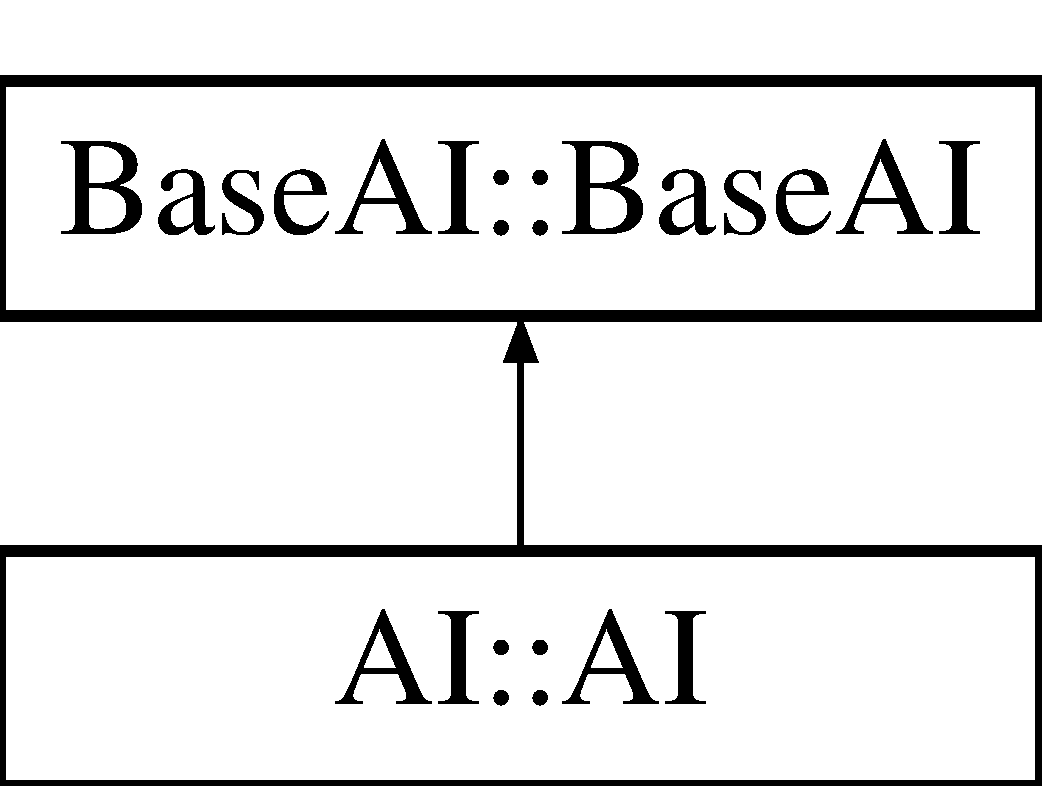
\includegraphics[height=2.000000cm]{classAI_1_1AI}
\end{center}
\end{figure}
\subsection*{Public Member Functions}
\begin{DoxyCompactItemize}
\item 
\hypertarget{classAI_1_1AI_a1173d35565e571260327628b5fdbf601}{
def {\bfseries username}}
\label{classAI_1_1AI_a1173d35565e571260327628b5fdbf601}

\item 
\hypertarget{classAI_1_1AI_a0c68d55972c20f5b5c12b3413dccf4f8}{
def {\bfseries password}}
\label{classAI_1_1AI_a0c68d55972c20f5b5c12b3413dccf4f8}

\item 
\hypertarget{classAI_1_1AI_abe85fa052f61e71327d0f066866360ec}{
def {\bfseries init}}
\label{classAI_1_1AI_abe85fa052f61e71327d0f066866360ec}

\item 
\hypertarget{classAI_1_1AI_a42dd3d0b74c0e3aae12c5d6165ec1d37}{
def {\bfseries end}}
\label{classAI_1_1AI_a42dd3d0b74c0e3aae12c5d6165ec1d37}

\item 
\hypertarget{classAI_1_1AI_a0e95ce8db48896cbf1dcf410930ca141}{
def {\bfseries run}}
\label{classAI_1_1AI_a0e95ce8db48896cbf1dcf410930ca141}

\item 
\hypertarget{classAI_1_1AI_afc336c04d31701982b4aa115de277f2a}{
def {\bfseries \_\-\_\-init\_\-\_\-}}
\label{classAI_1_1AI_afc336c04d31701982b4aa115de277f2a}

\end{DoxyCompactItemize}


\subsection{Detailed Description}
\begin{DoxyVerb}The class implementing gameplay logic.\end{DoxyVerb}
 

The documentation for this class was generated from the following file:\begin{DoxyCompactItemize}
\item 
AI.py\end{DoxyCompactItemize}

\hypertarget{classBaseAI_1_1BaseAI}{
\section{BaseAI::BaseAI Class Reference}
\label{classBaseAI_1_1BaseAI}\index{BaseAI::BaseAI@{BaseAI::BaseAI}}
}
Inheritance diagram for BaseAI::BaseAI:\begin{figure}[H]
\begin{center}
\leavevmode
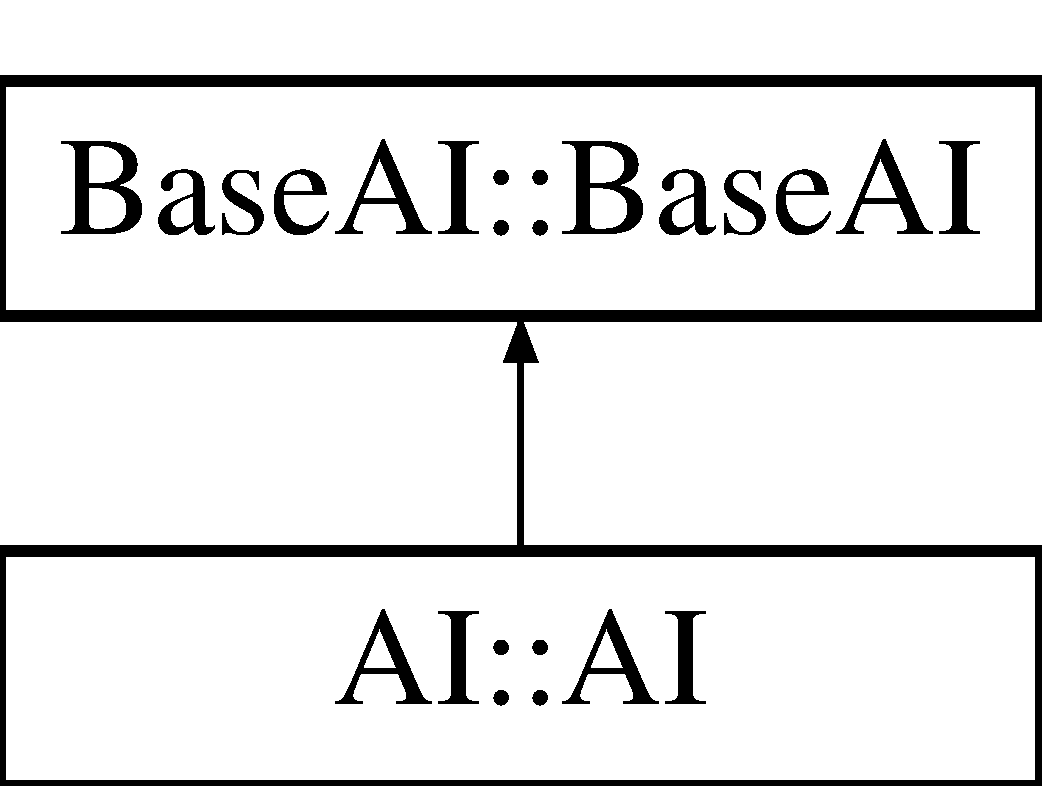
\includegraphics[height=2.000000cm]{classBaseAI_1_1BaseAI}
\end{center}
\end{figure}
\subsection*{Public Member Functions}
\begin{DoxyCompactItemize}
\item 
\hypertarget{classBaseAI_1_1BaseAI_a2dcbc8732112a39869c75ed9f0771633}{
def {\bfseries startTurn}}
\label{classBaseAI_1_1BaseAI_a2dcbc8732112a39869c75ed9f0771633}

\item 
\hypertarget{classBaseAI_1_1BaseAI_afa3d3ad590dd453c4d064a3c16b7f1a8}{
def {\bfseries turnNumber}}
\label{classBaseAI_1_1BaseAI_afa3d3ad590dd453c4d064a3c16b7f1a8}

\item 
\hypertarget{classBaseAI_1_1BaseAI_a60e0d6b3832faae7c85b4c9f0be10196}{
def {\bfseries playerID}}
\label{classBaseAI_1_1BaseAI_a60e0d6b3832faae7c85b4c9f0be10196}

\item 
\hypertarget{classBaseAI_1_1BaseAI_a32416775fed0eb83efe7221d732cbd70}{
def {\bfseries gameNumber}}
\label{classBaseAI_1_1BaseAI_a32416775fed0eb83efe7221d732cbd70}

\item 
\hypertarget{classBaseAI_1_1BaseAI_ac44d94ca17f3f274d124bdfd14f14031}{
def {\bfseries TurnsToStalemate}}
\label{classBaseAI_1_1BaseAI_ac44d94ca17f3f274d124bdfd14f14031}

\item 
\hypertarget{classBaseAI_1_1BaseAI_a3bf925534912eaebc263179a9c058f17}{
def {\bfseries player0Time}}
\label{classBaseAI_1_1BaseAI_a3bf925534912eaebc263179a9c058f17}

\item 
\hypertarget{classBaseAI_1_1BaseAI_a947dcca2869c60f33dbb3b553d70a321}{
def {\bfseries player1Time}}
\label{classBaseAI_1_1BaseAI_a947dcca2869c60f33dbb3b553d70a321}

\item 
\hypertarget{classBaseAI_1_1BaseAI_a0b938d864530091b6efd420a2ed38d10}{
def {\bfseries \_\-\_\-init\_\-\_\-}}
\label{classBaseAI_1_1BaseAI_a0b938d864530091b6efd420a2ed38d10}

\end{DoxyCompactItemize}
\subsection*{Static Public Attributes}
\begin{DoxyCompactItemize}
\item 
\hypertarget{classBaseAI_1_1BaseAI_a32a836eb9aad27c111583f24238a686c}{
{\bfseries initialized} = False}
\label{classBaseAI_1_1BaseAI_a32a836eb9aad27c111583f24238a686c}

\item 
\hypertarget{classBaseAI_1_1BaseAI_a54d7182ce68d3d2b55d247c431561f9d}{
int {\bfseries iteration} = 0}
\label{classBaseAI_1_1BaseAI_a54d7182ce68d3d2b55d247c431561f9d}

\item 
\hypertarget{classBaseAI_1_1BaseAI_af78c73cdbcca5a8ed213e2510fbd6e94}{
{\bfseries runGenerator} = None}
\label{classBaseAI_1_1BaseAI_af78c73cdbcca5a8ed213e2510fbd6e94}

\item 
\hypertarget{classBaseAI_1_1BaseAI_a319a81bb1af508789e826e78ee727418}{
{\bfseries connection} = None}
\label{classBaseAI_1_1BaseAI_a319a81bb1af508789e826e78ee727418}

\item 
\hypertarget{classBaseAI_1_1BaseAI_a9106a04e624e5f0da99f5bda529e59a2}{
list {\bfseries moves} = \mbox{[}$\,$\mbox{]}}
\label{classBaseAI_1_1BaseAI_a9106a04e624e5f0da99f5bda529e59a2}

\item 
\hypertarget{classBaseAI_1_1BaseAI_a1a0a022fb350336d7903bb86b25db1cf}{
list {\bfseries pieces} = \mbox{[}$\,$\mbox{]}}
\label{classBaseAI_1_1BaseAI_a1a0a022fb350336d7903bb86b25db1cf}

\end{DoxyCompactItemize}


\subsection{Detailed Description}
\begin{DoxyVerb}@brief A basic AI interface.

This class implements most the code an AI would need to interface with the lower-level game code.
AIs should extend this class to get a lot of builer-plate code out of the way
The provided AI class does just that.
\end{DoxyVerb}
 

The documentation for this class was generated from the following file:\begin{DoxyCompactItemize}
\item 
BaseAI.py\end{DoxyCompactItemize}

\hypertarget{classExistentialError_1_1ExistentialError}{
\section{ExistentialError::ExistentialError Class Reference}
\label{classExistentialError_1_1ExistentialError}\index{ExistentialError::ExistentialError@{ExistentialError::ExistentialError}}
}


The documentation for this class was generated from the following file:\begin{DoxyCompactItemize}
\item 
ExistentialError.py\end{DoxyCompactItemize}

\hypertarget{classGameObject_1_1GameObject}{
\section{GameObject::GameObject Class Reference}
\label{classGameObject_1_1GameObject}\index{GameObject::GameObject@{GameObject::GameObject}}
}
Inheritance diagram for GameObject::GameObject:\begin{figure}[H]
\begin{center}
\leavevmode
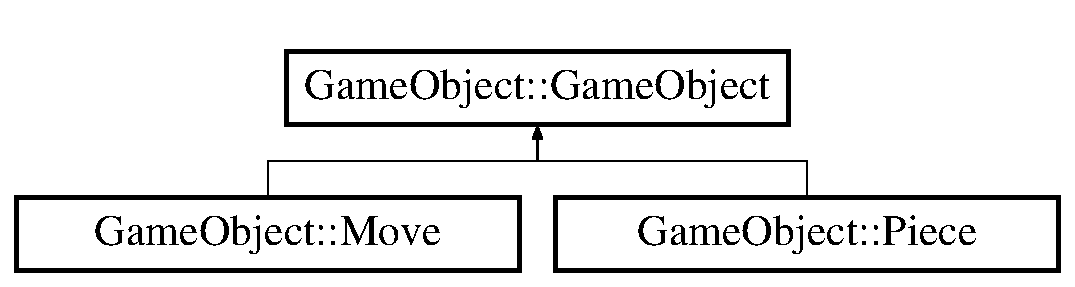
\includegraphics[height=2.000000cm]{classGameObject_1_1GameObject}
\end{center}
\end{figure}
\subsection*{Public Member Functions}
\begin{DoxyCompactItemize}
\item 
\hypertarget{classGameObject_1_1GameObject_ab8fc51fb12907dfeb24e3396eff13252}{
def {\bfseries \_\-\_\-init\_\-\_\-}}
\label{classGameObject_1_1GameObject_ab8fc51fb12907dfeb24e3396eff13252}

\end{DoxyCompactItemize}
\subsection*{Public Attributes}
\begin{DoxyCompactItemize}
\item 
\hypertarget{classGameObject_1_1GameObject_ab09e368639157c6fa81535684ad600db}{
{\bfseries ptr}}
\label{classGameObject_1_1GameObject_ab09e368639157c6fa81535684ad600db}

\item 
\hypertarget{classGameObject_1_1GameObject_a36654bebef12ac56a2abf4988bb49c95}{
{\bfseries iteration}}
\label{classGameObject_1_1GameObject_a36654bebef12ac56a2abf4988bb49c95}

\end{DoxyCompactItemize}


The documentation for this class was generated from the following file:\begin{DoxyCompactItemize}
\item 
GameObject.py\end{DoxyCompactItemize}

\hypertarget{classGameObject_1_1Move}{
\section{GameObject::Move Class Reference}
\label{classGameObject_1_1Move}\index{GameObject::Move@{GameObject::Move}}
}


A chess move.  


Inheritance diagram for GameObject::Move:\begin{figure}[H]
\begin{center}
\leavevmode
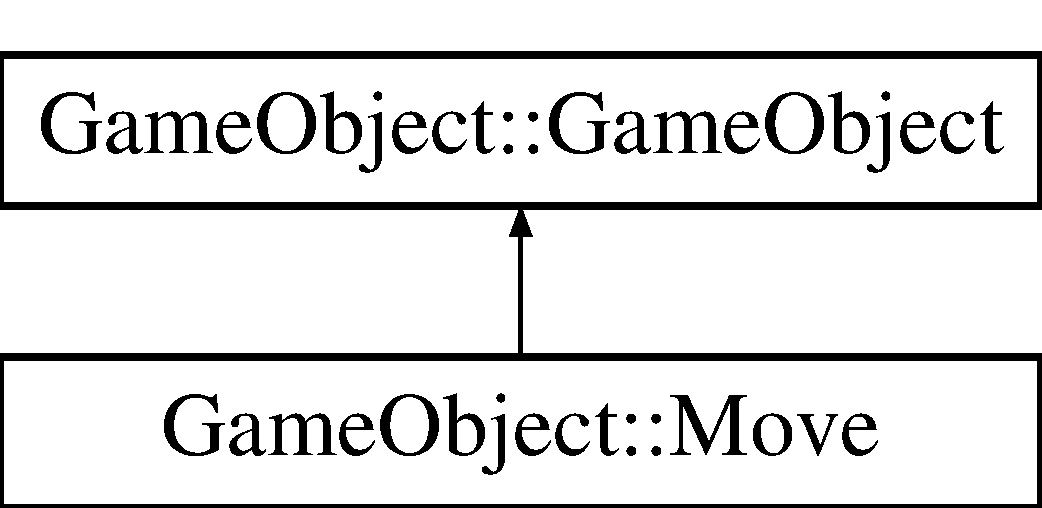
\includegraphics[height=2.000000cm]{classGameObject_1_1Move}
\end{center}
\end{figure}
\subsection*{Public Member Functions}
\begin{DoxyCompactItemize}
\item 
\hypertarget{classGameObject_1_1Move_a28c1b754287122156ba6cadd330cfc7a}{
def {\bfseries \_\-\_\-init\_\-\_\-}}
\label{classGameObject_1_1Move_a28c1b754287122156ba6cadd330cfc7a}

\item 
\hypertarget{classGameObject_1_1Move_aecb61e2c300b06205b74d47d3e1faa8e}{
def {\bfseries validify}}
\label{classGameObject_1_1Move_aecb61e2c300b06205b74d47d3e1faa8e}

\item 
\hypertarget{classGameObject_1_1Move_adde9eb54c013b37df51bdde531827ecb}{
def \hyperlink{classGameObject_1_1Move_adde9eb54c013b37df51bdde531827ecb}{getId}}
\label{classGameObject_1_1Move_adde9eb54c013b37df51bdde531827ecb}

\begin{DoxyCompactList}\small\item\em Unique Identifier. \item\end{DoxyCompactList}\item 
\hypertarget{classGameObject_1_1Move_a58418b0ccdb8c6e5bddc27332895802f}{
def \hyperlink{classGameObject_1_1Move_a58418b0ccdb8c6e5bddc27332895802f}{getFromFile}}
\label{classGameObject_1_1Move_a58418b0ccdb8c6e5bddc27332895802f}

\begin{DoxyCompactList}\small\item\em The initial file location. \item\end{DoxyCompactList}\item 
\hypertarget{classGameObject_1_1Move_a492534bd34612e25043c70df14722826}{
def \hyperlink{classGameObject_1_1Move_a492534bd34612e25043c70df14722826}{getFromRank}}
\label{classGameObject_1_1Move_a492534bd34612e25043c70df14722826}

\begin{DoxyCompactList}\small\item\em The initial rank location. \item\end{DoxyCompactList}\item 
\hypertarget{classGameObject_1_1Move_a20f7d1d252fb96aa80c356f44badf880}{
def \hyperlink{classGameObject_1_1Move_a20f7d1d252fb96aa80c356f44badf880}{getToFile}}
\label{classGameObject_1_1Move_a20f7d1d252fb96aa80c356f44badf880}

\begin{DoxyCompactList}\small\item\em The final file location. \item\end{DoxyCompactList}\item 
\hypertarget{classGameObject_1_1Move_ab4274abab85fdc4567d5e454ec920849}{
def \hyperlink{classGameObject_1_1Move_ab4274abab85fdc4567d5e454ec920849}{getToRank}}
\label{classGameObject_1_1Move_ab4274abab85fdc4567d5e454ec920849}

\begin{DoxyCompactList}\small\item\em The final rank location. \item\end{DoxyCompactList}\item 
def \hyperlink{classGameObject_1_1Move_a615ace235019328089cca1a1f8674955}{getPromoteType}
\begin{DoxyCompactList}\small\item\em The type of the piece for pawn promotion. \item\end{DoxyCompactList}\item 
\hypertarget{classGameObject_1_1Move_a23d509a282101220907d2438918be680}{
def {\bfseries \_\-\_\-str\_\-\_\-}}
\label{classGameObject_1_1Move_a23d509a282101220907d2438918be680}

\end{DoxyCompactItemize}
\subsection*{Public Attributes}
\begin{DoxyCompactItemize}
\item 
\hypertarget{classGameObject_1_1Move_a6d3e5a3f5e8875c18bce3cd43e5e8c7f}{
{\bfseries ptr}}
\label{classGameObject_1_1Move_a6d3e5a3f5e8875c18bce3cd43e5e8c7f}

\item 
\hypertarget{classGameObject_1_1Move_a516e4b67ebe588c76b955221d3fc1659}{
{\bfseries iteration}}
\label{classGameObject_1_1Move_a516e4b67ebe588c76b955221d3fc1659}

\item 
\hypertarget{classGameObject_1_1Move_ad61e6afdc612d8005a6117ce4061efad}{
{\bfseries id}}
\label{classGameObject_1_1Move_ad61e6afdc612d8005a6117ce4061efad}

\end{DoxyCompactItemize}


\subsection{Detailed Description}
A chess move. 

\subsection{Member Function Documentation}
\hypertarget{classGameObject_1_1Move_a615ace235019328089cca1a1f8674955}{
\index{GameObject::Move@{GameObject::Move}!getPromoteType@{getPromoteType}}
\index{getPromoteType@{getPromoteType}!GameObject::Move@{GameObject::Move}}
\subsubsection[{getPromoteType}]{\setlength{\rightskip}{0pt plus 5cm}def GameObject::Move::getPromoteType (
\begin{DoxyParamCaption}
\item[{}]{ self}
\end{DoxyParamCaption}
)}}
\label{classGameObject_1_1Move_a615ace235019328089cca1a1f8674955}


The type of the piece for pawn promotion. 

Q=Queen, B=Bishop, N=Knight, R=Rook 

The documentation for this class was generated from the following file:\begin{DoxyCompactItemize}
\item 
GameObject.py\end{DoxyCompactItemize}

\hypertarget{classGameObject_1_1Piece}{
\section{GameObject::Piece Class Reference}
\label{classGameObject_1_1Piece}\index{GameObject::Piece@{GameObject::Piece}}
}


A chess piece.  


Inheritance diagram for GameObject::Piece:\begin{figure}[H]
\begin{center}
\leavevmode
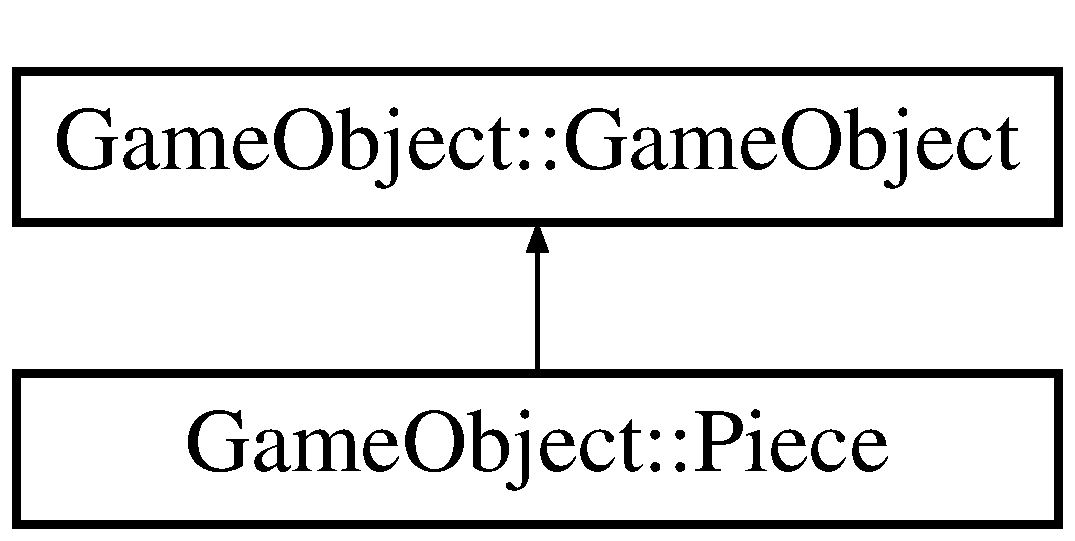
\includegraphics[height=2.000000cm]{classGameObject_1_1Piece}
\end{center}
\end{figure}
\subsection*{Public Member Functions}
\begin{DoxyCompactItemize}
\item 
\hypertarget{classGameObject_1_1Piece_a02e3b426bffb9b78351db4db2e96110e}{
def {\bfseries \_\-\_\-init\_\-\_\-}}
\label{classGameObject_1_1Piece_a02e3b426bffb9b78351db4db2e96110e}

\item 
\hypertarget{classGameObject_1_1Piece_a785939a2ed9095faf1f89313fbe2ed4f}{
def {\bfseries validify}}
\label{classGameObject_1_1Piece_a785939a2ed9095faf1f89313fbe2ed4f}

\item 
\hypertarget{classGameObject_1_1Piece_a51f8b88edc75d146cbca63544942cd19}{
def {\bfseries move}}
\label{classGameObject_1_1Piece_a51f8b88edc75d146cbca63544942cd19}

\item 
\hypertarget{classGameObject_1_1Piece_a99894fa06f43444aab3c9e2f9cf2cf7e}{
def \hyperlink{classGameObject_1_1Piece_a99894fa06f43444aab3c9e2f9cf2cf7e}{getId}}
\label{classGameObject_1_1Piece_a99894fa06f43444aab3c9e2f9cf2cf7e}

\begin{DoxyCompactList}\small\item\em Unique Identifier. \item\end{DoxyCompactList}\item 
\hypertarget{classGameObject_1_1Piece_af92af15f1eb2ce4c5904a86dee91e0cb}{
def \hyperlink{classGameObject_1_1Piece_af92af15f1eb2ce4c5904a86dee91e0cb}{getOwner}}
\label{classGameObject_1_1Piece_af92af15f1eb2ce4c5904a86dee91e0cb}

\begin{DoxyCompactList}\small\item\em The owner of the piece. \item\end{DoxyCompactList}\item 
\hypertarget{classGameObject_1_1Piece_a0178c97d2cda992d5d80a767c7462994}{
def \hyperlink{classGameObject_1_1Piece_a0178c97d2cda992d5d80a767c7462994}{getFile}}
\label{classGameObject_1_1Piece_a0178c97d2cda992d5d80a767c7462994}

\begin{DoxyCompactList}\small\item\em The letter this piece is at (1-\/8). \item\end{DoxyCompactList}\item 
\hypertarget{classGameObject_1_1Piece_a0a58cac3e57264a2b1ce723866009a0c}{
def \hyperlink{classGameObject_1_1Piece_a0a58cac3e57264a2b1ce723866009a0c}{getRank}}
\label{classGameObject_1_1Piece_a0a58cac3e57264a2b1ce723866009a0c}

\begin{DoxyCompactList}\small\item\em The number this piece is at (1-\/8). \item\end{DoxyCompactList}\item 
\hypertarget{classGameObject_1_1Piece_a3ddf1a9b0feb735b4c6d6133f3f935e7}{
def \hyperlink{classGameObject_1_1Piece_a3ddf1a9b0feb735b4c6d6133f3f935e7}{getHasMoved}}
\label{classGameObject_1_1Piece_a3ddf1a9b0feb735b4c6d6133f3f935e7}

\begin{DoxyCompactList}\small\item\em 1=has moved, 0=has not moved \item\end{DoxyCompactList}\item 
def \hyperlink{classGameObject_1_1Piece_aada307c3b0bd9830613b8ef70c6eebc3}{getType}
\begin{DoxyCompactList}\small\item\em The letter that describes this piece's type. \item\end{DoxyCompactList}\item 
\hypertarget{classGameObject_1_1Piece_ac535f7b06749009aac49367528b7d746}{
def {\bfseries \_\-\_\-str\_\-\_\-}}
\label{classGameObject_1_1Piece_ac535f7b06749009aac49367528b7d746}

\end{DoxyCompactItemize}
\subsection*{Public Attributes}
\begin{DoxyCompactItemize}
\item 
\hypertarget{classGameObject_1_1Piece_a7e8c2348f727cf54c4332364997e0186}{
{\bfseries ptr}}
\label{classGameObject_1_1Piece_a7e8c2348f727cf54c4332364997e0186}

\item 
\hypertarget{classGameObject_1_1Piece_a41bd4f862bda543aed6462ad17a13758}{
{\bfseries iteration}}
\label{classGameObject_1_1Piece_a41bd4f862bda543aed6462ad17a13758}

\item 
\hypertarget{classGameObject_1_1Piece_a05d8f7aff1663c0bd46f201cae3f7070}{
{\bfseries id}}
\label{classGameObject_1_1Piece_a05d8f7aff1663c0bd46f201cae3f7070}

\end{DoxyCompactItemize}


\subsection{Detailed Description}
A chess piece. 

\subsection{Member Function Documentation}
\hypertarget{classGameObject_1_1Piece_aada307c3b0bd9830613b8ef70c6eebc3}{
\index{GameObject::Piece@{GameObject::Piece}!getType@{getType}}
\index{getType@{getType}!GameObject::Piece@{GameObject::Piece}}
\subsubsection[{getType}]{\setlength{\rightskip}{0pt plus 5cm}def GameObject::Piece::getType (
\begin{DoxyParamCaption}
\item[{}]{ self}
\end{DoxyParamCaption}
)}}
\label{classGameObject_1_1Piece_aada307c3b0bd9830613b8ef70c6eebc3}


The letter that describes this piece's type. 

K=King, Q=Queen, B=Bishop, N=Knight, R=Rook, P=Pawn 

The documentation for this class was generated from the following file:\begin{DoxyCompactItemize}
\item 
GameObject.py\end{DoxyCompactItemize}

\printindex
\end{document}
